\documentclass{aamas2014}

\usepackage{amssymb}
\usepackage{graphicx}
\usepackage{epstopdf}
\usepackage{multirow}
\usepackage{url,eqnarray,amsmath,amssymb,epsfig,verbatim}
\usepackage{tikz}
\usepackage{subfig}
\usepackage{booktabs}
\usetikzlibrary{matrix,arrows,decorations.pathmorphing,backgrounds,shadows,positioning}
\usepackage{pgfplots}
\usepackage{filecontents}
\pdfpagewidth=8.5truein
\pdfpageheight=11truein

\providecommand{\customsubsub}[1]{~\\[-0.7em]\noindent{\bf {#1.}}}
%%some notation
\providecommand{\E}{\mathbb{E}}
\providecommand{\SALEP}{SALE POMDP}
\providecommand{\NoAQ}{\textsc{NoAQ}}
\newlength{\EqSpace}
\setlength{\EqSpace}{-9mm}


\makeatletter
 \let\@copyrightspace\relax
 \makeatother
\begin{document}


\title{A POMDP Based Approach to Optimally Select Sellers in E-Marketplaces}

\author{Paper XXX}

\maketitle

\begin{abstract}
In e-marketplaces, buying agents choose among multiple sellers, finding the best one to perform a transaction. A seller's quality is mainly determined using buyers' assessments on the seller based on previous transactions. How a buyer utilizes existing information and chooses the right seller, while maximizing its utility derived from the decision process is crucial, since the value derived from a successful transaction with the seller, may be negligible relative to the cost of choosing the right seller. This paper presents \SALEP{}, a framework based on the \textit{Partially Observable Markov Decision Process}, which helps a buyer to optimally select the right seller to perform a transaction. The framework is robust in the sense that it also allows to reason about the quality of other buying agents (advisors) in the market, who provide opinions about the sellers. Experimental results on the ART Testbed demonstrate that \SALEP{} can optimally select the right sellers and advisors (to ask opinions), effectively balancing the trade-off between the cost of obtaining and benefit of more information, than traditional trust models.
\end{abstract}

\category{I.2.11}{Distributed Artificial Intelligence}{Intelligent Agents; Multiagent Systems}

\terms{Performance; Design}

\keywords{Seller Selection, E-Marketplace, POMDPs.}

\section{Introduction}\label{introduction}

In multi-agent based e-marketplaces, self-interested selling agents can act maliciously by not delivering products with the same quality as promised. It is thus important for buying agents to analyze the quality of sellers and determine which sellers to do business with. Buyers maintain beliefs over the quality levels of the sellers, based on their previous transactions, using which they may select the best seller to interact with. However, realistically, in most e-marketplaces, buyers often encounter sellers with which they have no previous experience. In such cases, they can query other buyers (called advisors) about their beliefs on the sellers' quality.

A number of trust models (\textit{e.g.} BRS~\cite{whitby05}, TRAVOS~\cite{teach06}, Personalized~\cite{zhang09thesis}, BLADE~\cite{regan2006bayesian}, etc.), have been proposed by researchers in the multi-agent community to help buyers assess seller quality and choose transaction partners. These approaches work by combining the buyer's own belief and those of the advisors, to estimate the true quality of the seller. However, the above approaches mainly focus on accurately estimating the quality of the seller rather than optimally choosing a right seller to perform transaction with. This is because the above trust models fail to reason \textit{when} it is necessary to query advisors, though they may determine \textit{whom} to query by analyzing the quality levels (trustworthiness) of the advisors. Most approaches simply query all advisors who have interacted with the seller. This will in fact result in negligible utility for the buyer, especially when the querying advisors are large in numbers, since the cost of querying advisors may be greater than the value derived from a successful transaction with the seller.

Regan \textit{et al.}~\cite{regan2005advisor} proposed the \textit{Advisor} POMDP, which considers the seller selection problem as a \textit{Partially Observable Markov Decision Process}. POMDPs provide a framework for making optimal decisions in partially observable environments~\cite{kaelbling1998planning}. The main advantage of using POMDPs is that  rather than trying to achieve the most accurate estimate of sellers, the approach tries to select good sellers and does that optimally. However, \textit{Advisor} POMDP did not reason about advisors' quality levels and considered all advisors to be trustworthy.  Also, in \textit{Advisor} POMDP, each advisor provides opinions about its beliefs on all sellers, when queried, resulting in a lot of unnecessary information. Rather than estimating the quality of all sellers, the only goal should be to select the seller with high quality.

In this paper, we present SALE (\emph{(S)eller \& (A)dvisor se(LE)ction}) POMDP~\cite{oliehoekreasoning}, a framework to deal with the seller selection problem in an effective manner. Here, the buying agent is modeled as a POMDP, with the main goal of optimally selecting the right seller to perform a transaction. In this process, it maintains beliefs over the quality levels of sellers, as well as that of advisors. To query advisors about the quality of the sellers, it firstly determines the trustworthiness of the advisors, thereby limiting its interactions to the honest ones. It also makes provision to query advisors about their beliefs on other advisors, sufficiently using it to improve its own beliefs and make optimal decisions, especially in sophisticated attacking scenarios. It can also account for the buyers' experience in the market by considering the influence of previous responses (history) in the POMDP formulation.  \SALEP{} can also be modeled as a \textit{factored} POMDP to resolve the scalability issues, which is a limiting factor in solving most POMDPs~\cite{poupart2005exploiting}. In this paper, we conducted a thorough evaluation of \SALEP{} using the ART testbed to prove the effectiveness of \SALEP{} against traditional trust models in optimally selecting sellers, even in the presence of strategic attacks.


The rest of the paper is organized as follows. Section~\ref{sec:2} gives a brief discussion of existing trust models and explains \textit{Advisor} POMDP in detail. The detailed description of the \SALEP\ model is present in Section~\ref{sec:3}, which also discusses the \textit{factored} nature of \SALEP{}. In Section~\ref{sec:5}, we conduct an extensive experimentation of \SALEP{} using the ART testbed, and demonstrate the effectiveness of \SALEP\ in optimally selecting the right sellers to perform transaction with. The scalability of the \textit{factored} approach is also analyzed. Finally, Section~\ref{sec:6} concludes the current work and proposes future work.

\section{Background}\label{sec:2}
\subsection{Trust Models}
Many trust models have been proposed in literature to address the seller selection problem. Reputation System (BRS)~\cite{whitby05} models the seller's reputation as the expected value of the beta probability distribution of the trusted advisors' beliefs about the seller. Teacy \emph{et al.}~\cite{teach06} propose TRAVOS which is also based on beta probability distribution. It integrates a buyer's own beliefs about sellers as well as the beliefs of advisors to determine seller's quality. The personalized approach~\cite{zhang08}, models seller's quality as a weighted score of its public and private reputation which is based on the buyer's own experience and that of the advisors respectively. The BLADE approach of Regan et al.~\cite{regan2006bayesian} allows a buyer to learn other advisors' evaluation functions on different features of the services delivered by sellers, by which it can reinterpret advisors' beliefs instead of filtering them. However, all the above trust models do not provide optimal decision making for the buyer on whether and from which seller to perform transaction, which is exactly what our approach tries to offer.
\subsection{Advisor POMDP}
Regan \textit{et al.}~\cite{regan2005advisor} introduced the Advisor POMDP, an approach for dealing with the
seller section problem based on the POMDP framework. Partially observable Markov decision processes (POMDPs) provide a natural model for sequential decision making under uncertainty. A POMDP agent works towards the main goal of maximizing the expected discounted future reward~\cite{kaelbling1998planning} (buyers' utility in this case).  Formally, an Advisor POMDP consists of the following elements: If there are $I$ advisors that can be queried about the reputation of all $J$ sellers then,
\begin{itemize}
\item $\mathcal{S}$---a set of possible states of the environment. A state $s=\left\langle \vec{q},sat\right\rangle $, where $\vec{q}\in[0,1]^{J}$ is a vector indicating the quality $q_j$ of each seller and $sat\in\left\{ -1,0,+1\right\} $ indicates the result of a purchase: satisfactory ($+1$), unsatisfactory ($-1$) or whether no purchase took place yet~(0).
\item $\mathcal{A}$---a set of actions. There is one action $ask_{i}$ for each advisor~$i$, and one $buy_{j}$ action for each seller~$j$.
\item $T$---a transition function that specifies $\Pr(s'|s,a)$, the probability of transferring to a state $s'$ given that action $a$ was taken in state $s$. For $ask_i$ actions, the state does not change. For $buy_{j}$ action a state $s=\left\langle \vec{q},0\right\rangle $ changes stochastically to $s'=\left\langle \vec{q},-1\right\rangle $ or $s=\left\langle \vec{q},+1\right\rangle $ with probabilities depending on ${q}_{j}$.
\item $R$---a reward function specifying $R(s,a,s')$. For ask actions, a small cost is paid. For transitions to a satisfied state (i.e., from $sat=0$ to $sat=+1$) a reward is received, while transitions to an unsatisfied state yield a large penalty. Once the state has changed to satisfied or unsatisfied, no further rewards are given.
\item $\Omega$---a set of observations~$o$. In the advisor POMDP, the advisors respond with a tuple $o=\left\langle rep_{j},cf_{j}\right\rangle _{j=1}^{J}$ that expresses the knowledge of that advisor about all sellers. Here $rep_{j}$ is the reputation according to the advisor and $cf_{j}$ is a measure of its certainty.
\item $O$---the observation function that specifies $\Pr(o|a,s)$. Since the semantics of the certainty factors are not formalized, there is some freedom in its specification.
\item $b^{0}$---the initial state distribution.
\item $h$---the \emph{horizon} of the problem. That is the number of time steps, or \emph{stages}, for which we want to plan. $h$ can also be infinite.
\end{itemize}

However, \textit{Advisor} POMDP does not consider advisor's quality to be a part of the state space, making it vulnerable to unfair rating attacks~\cite{irissappane2012towards}, where advisors may provide incorrect opinions about sellers. Also observations in \textit{Advisor} POMDP contain beliefs about all sellers, resulting in an unnecessary exchange of information during the $ask$ actions.

%\section{Related Work}\label{sec:2}
%
%
%Many trust models have been proposed in literature to address the seller selection problem. They model sellers' quality (reputation), using opinions from other buyers and thereby select the best seller to interact with. The Beta Reputation System (BRS)~\cite{whitby05} models the seller's reputation as the expected value of the beta probability distribution of the trusted advisors' beliefs about the seller. If the calculated reputation of a seller based on the opinions from the set of honest buyers falls within the rejection area ($q$ quantile or $1-q$ quantile) of the beta distribution of an advisor's beliefs on the seller, then the advisor is considered untrustworthy. BRS is a centralized approach and is heavily based on the \textit{majority rule}. Teacy \emph{et al.}~\cite{teach06} propose TRAVOS which is also based on beta probability distribution. To calculate the reputation of a seller, it integrates buyer's own beliefs about sellers as well as the beliefs of advisors, after assessing their credibility. The personalized approach~\cite{zhang08}, models seller's quality as a weighted score of its public and private reputation. The private reputation is calculated as the expected value of the beta probability distribution of the buyer's beliefs on the seller and the public reputation is calculated using the beliefs of the advisors, after discounting them based on their trustworthiness. However, it assumes the behavior of the advisors to be consistent across all sellers.
%
%The BLADE approach of Regan et al.~\cite{regan2006bayesian} applies Bayesian learning to reinterpret advisors' beliefs instead of filtering them. The BLADE model allows a buyer to learn other advisors' evaluation functions on different features of the services delivered by sellers, by analyzing their beliefs. This makes it possible to adjust the advisor's beliefs, thereby coping with subjectivity and deception, while determining the quality of the seller. However, the model assumes consistent advisor behavior and also requires multiple transactions with the same seller to accurately interpret its quality. In contrast, in \SALEP\ we learn about advisors by asking other advisors, thereby avoiding the need to engage in costly transactions. Also, all the above trust models do not provide optimal decision making for the buyer on whether and from which seller to perform transaction, which is exactly what our approach tries to offer.
%
%Few works based on POMDPs exist to address the seller selection problem using the notion of trust. The \textit{Advisor} POMDP~\cite{regan2005advisor}, described by $\left\langle \mathcal{S},\mathcal{A},\mathcal{T},\mathcal{R},\Omega,\mathcal{O}\right\rangle$, where $\mathcal{S}$ represents the possible states consisting of the seller's quality and the outcome of the transaction with seller, $\mathcal{A}$ represents the actions $\in {ask, buy}$, $\mathcal{T}$ represents the transition functions, $\mathcal{R}$ represents the rewards based on the outcomes of the transaction, $\Omega$ represents the observations from advisors, consisting of the advisors' beliefs about the sellers along with the certainty and $\mathcal{O}$ denotes the observation function, updates its belief about the seller via Bayes' rule, on interacting with other advisors in the environment, thereby selecting the right seller to perform transaction. However, \textit{Advisor} POMDP does not consider advisor's quality to be a part of the state space, making it vulnerable to unfair rating attacks. Also the observations in \textit{Advisor} POMDP contain beliefs about all sellers, resulting in an unnecessary exchange of information during the $ask$ actions. Seymour \textit{et al.}~\cite{seymour2009trust} proposed TI-POMDP, which adds trust modeling to the I(interactive)-POMDP framework~\cite{gmytrasiewicz2005framework}. I-POMDP is a multi-agent extension of the POMDP framework, in which each agent maintains beliefs about both the physical states of the world and the decision process models of the other agents. The TI-POMDP maintains the basic components of the I-POMDP, and adds trust modeling as a primary decision factor for the agents. In addition to the state belief model, an agent maintains and updates a trust model (a rating of the trustworthiness of the other agents) for the environment. This trust model contains an agent's level of trust in the other agents, which helps to decide whether or not to cooperate with another agent on a given task. However, this model depends heavily on communication between the agents for decidability~\cite{mayo2010multi}. Whereas, in our work, we aim to optimally select the sellers, under conditions of uncertainty, by securing additional information on the seller's (and advisor's) quality levels from other agents in the market, eliminating the need to explicitly engage in personal interactions with the sellers.

\section{The \SALEP{} Model}\label{sec:3}
\subsection{Basic \SALEP{}}
In this section, we introduce the \SALEP{} model for dealing with the seller section problem by optimally selecting the right seller to perform transaction (rather than accurately determining the quality of the sellers). Unlike \textit{Advisor} POMDP, \SALEP{} assumes that advisors also have quality levels (\emph{trustworthiness}) and considers it as part of the state space. It also allows agents to query about the quality of other advisors in the system. Each \SALEP{} agent can be described in terms of states, actions, observations and rewards such that:
\begin{itemize}
\item $\mathcal{S}$---a set of possible states of the environment. A state contains the quality levels\footnote{we assume discrete quality levels, in order to use standard POMDP solvers.} of each seller, advisor and the status of the current transaction. Let $\mathcal{Q}$ be the discrete set of seller quality levels and $\mathcal{U}$ be the set of advisor quality levels. Then, a state is a tuple $s=\left\langle \vec{q},\vec{u},sat\right\rangle $, where $\vec{q}\in\mathcal{Q}^{J}$ is a vector indicating the quality of each seller, $\vec{u}\in\mathcal{U}^{I}$ a vector indicating the quality of each advisor, and $sat$ indicates the status of the current transaction, which can be $not\_started$, $satisfactory$, $unsatisfactory$, $gave\_up$ or $finished$. We also write $q_{j}$ for the $j$-th element of $\vec{q}$ and $u_{i}$ for the $i$-th element of $\vec{u}$. The decision process begins when $sat = not\_started$. The end of the decision process is modeled using sets of terminal states (such as $satisfactory, unsatisfactory, gave\_up$) \textit{i:e} $buy_j$ actions may result in a successful ($sat$ = $satisfactory$) or unsuccessful ($sat = unsatisfactory$) transaction and $do\_not\_buy$ action will result in $sat = gave\_up$. Any transitions from the terminal states will result in $sat = finished$.

\item $\mathcal{A}$---a set of actions which can be:\\[-1.8em]
        \begin{itemize}
            \item $seller\_query_{ij}$, ask advisor $i$ about seller~$j$,
            \item $advisor\_query_{ii'}$, ask advisor $i$ about advisor~$i'$,
            \item $buy_{j}$, buy from seller~$j$.
            \item $do\_not\_buy$, decide not to buy from any seller.
        \end{itemize}
    \vspace{-1em}
\item $T$---a transition function that specifies $\Pr(s'|s,a)$, the probability of transferring to a state $s'$ given that action $a$ was taken in state $s$. We assume that when taking a query action, the state does not change:
        \begin{equation}
            \forall_{i,j}\quad\Pr(s'|s,seller\_query_{ij})=\delta_{ss'}
        \end{equation}
        \\[\EqSpace]
        \begin{equation}
            \forall_{i,i'}\quad\Pr(s'|s,advisor\_query_{ii'})=\delta_{ss'}
        \end{equation}
    $\delta_{ss'}$ is the Kronecker delta \textit{i.e.} $1$ if and only if $s=s'$. When taking a $buy_{j}$ action, the state will always transition to a terminal state. The transition probabilities to terminal states give a definition of the quality levels. In general, chances of transition to \textit{satisfied} should be higher when buying from higher quality sellers. Together, the specifications of these transitions imply the assumption that quality and trust-levels are stationary for the duration of the decision process.

\item $R$---a reward function specifying $R(s,a,s')$: a small cost is associated with ask action $R(s,seller\_query_{ij})=R(s,advisor\_query_{ii'})=R_{ask}$; a reward is associated with a good purchase $R(s,buy_j,s'=\left\langle \vec{q},\vec{u},sat=+1\right\rangle )=R_{sat}$; a penalty is levied when the outcome of a transaction is \emph{unsatisfied} $R(s,buy_j,s'=\left\langle\vec{q},\vec{u},sat=-1\right\rangle )=R_{unsat}$ and for taking the $do\_not\_buy$ action when in fact there is a seller of high enough quality, otherwise there is a small reward for this action. Once the transaction state is \textit{satisfied}, \textit{unsatisfied} or \textit{gaveup}, no further rewards are given.
\item $\Omega$---a set of observations. When a \emph{query} action is performed the agent will receive an observation from the set of discriminated quality levels. That is, after a $seller\_query_{ij}$ action, the agent receives an observation $o\in \{good, bad\}$ corresponding to the quality of seller $j$, while after an $advisor\_query_{ii'}$ it will get an observation $o\in \{trustworthy, untrustworthy\}$ corresponding to the quality of advisor $i'$. When the agent transitions to a terminal state, it receives the observation \textit{ended}.
\item $O$---the observation function that specifies $\Pr(o|a,s)$. As in the Advisor POMDP, there is no a priori correct way to specify the observation probabilities. The probabilities picked for the observation function define the meaning of different trust levels. In general, the idea is that trustworthy advisors will give more accurate and consistent answers than untrustworthy ones.
\item $b^{0}$---the initial state distribution. It is dependent on the subjective beliefs of the agent, when the need for purchasing an item arises. For simplicity, one may start with a uniform belief over the quality levels, but a different initial belief can also be obtained as a result of previous interactions. That is, once the $buy_j$ or $do\_not\_buy$ action is performed, the resulting belief can be used as the basis for an initial belief for a new seller selection instantiation. In a bit more detail, There are two sources of previous experience: 1) previous seller selection tasks: the modified belief state resulting from advice in a previous problem can be retained and 2) actual experiences with sellers: even though in the decision making task we model a transition to a terminal state with a deterministic \emph{ended} observation, the actual order will result in the owner of the agent being satisfied or not and this information can be used to update the final belief of the agent's previous seller selection task giving a new initial belief for a new task\footnote{In fact this can be an important mechanism to deal with advisors that are consistent but deceptive and settings in which the majority of advisors is untrustworthy.}
\item $h$---the \emph{horizon} of the problem. That is the number of time steps, or \emph{stages}, for which we want to plan. We will assume that $h$ is infinite in this paper.
\end{itemize}
When the \SALEP{} agent interacts with the environment, it maintains a \emph{belief} $b$, i.e., a probability distribution over states via Bayes' rule. That is, when $b(s)$ specifies the probability of $s$ (for all $s$), we can derive $b'$ an updated belief after taking some action~$a$ and receiving an observation~$o$. Assuming discrete sets of states and observations, this update can be written as follows:
\begin{equation}
b'(s')\hspace{-1mm}=\hspace{-1mm}\frac{ \Pr(s',o|b,a) } {\Pr(o|b,a)}\
\hspace{-1mm}=\hspace{-1mm}\frac{1}{ \Pr(o|b,a) }
\Pr(o|a,s')
\sum_s
\Pr(s'|s,a)
b(s)
\label{eq:BU}
\end{equation}\\[-2mm]
Here, $\Pr(o|b,a)$ is a normalization factor.
%%SAVESPACE
%Regan et al.~\cite{Regan05PST} give a step by step illustration of the belief
%update in the continuous state case.

These beliefs are the basis for decision making: a policy $\pi$ maps beliefs to actions
$\pi(b)=a$. The goal of solving the POMDP is to find an optimal
policy that maximizes the expected discounted cumulative reward, also called
\emph{value}:\\[-2mm]
\begin{equation}
V(\pi)=\E\Big[\sum_{t=0}^{h-1} \gamma^t R(s,a,s') \mid \pi,b^0\Big],
\end{equation}\\[-3mm]
with $0\leq\gamma<1$ the discount factor.

Finding an optimal policy $\pi^*$ is intractable in general (PSPACE complete \cite{papadimitriou1987complexity}), however, in recent years substantial advances
have been made in approximate solutions (e.g.,~\cite{kurniawati2008sarsop,silver2010monte}). Since the \SALEP{} really is a \emph{factored} POMDP, we try and use solvers such as symbolic Perseus \cite{poupart2005exploiting} that exploit this property,  as discussed in the next section.

\subsection{Factored Representation}\label{sec:factored}

POMDPs with very large state spaces are impractical to be solved by the classic solution algorithms. However, such state spaces can be described using a set of state variables, and the effects of actions in terms of their effects on these variables. Dynamic Bayesian Networks (DBNs) with conditional probability tables (CPTs) in the form of decision-trees or
graphs are often used to represent these effects compactly referred to as a \textit{factored} representation~\cite{shani2013task}. Solvers such as Symbolic Perseus~\cite{poupart2005exploiting} exploit this \textit{factored} structure to resolve scalability issues in POMDPs.

To illustrate the \textit{factored} nature of the \SALEP{}, we will consider a simple case of the seller selection problem with $1$ seller and $2$ advisors such that $\mathcal{Q}=\left\{ L,H\right\} $, representing $L$(ow) and $H$(igh) seller quality and $\mathcal{U}=\left\{ T,U, A\right\} $, representing $T$(rustworty), $U$(ntrustworty) and $A$(dversarial) advisor quality levels, allowing to accommodate attacking behaviors: 1) $random$, where advisors provide random opinions; 2) $adversarial$, where advisors provide complimentary opinions. Each state $s \in \mathcal{S}$ is a compilation of the quality of each seller, quality of each advisor and transaction outcome, \textit{i.e.} $s=\left\langle \left\langle q_1\right\rangle, \left\langle u_1, u_2\right\rangle, sat\right\rangle$. To factor the \SALEP{} model, we decompose the transition and observation functions as follows.\\
 \textbf{Buy Action} The DBN and CPT for the $buy_{1}$ action  (buy from $s_1$) are shown in Fig~\ref{fig:BuyS1}. The probability of transferring to a state $s'$ given that action $buy_{1}$ was taken in state $s$ can be factored into a product of smaller conditional distributions with respect to its parent variables as shown in Eqn.~\ref{eq:buy}.  $\Pr(sat'|q'_1,sat,buy_{1})$ signifies that the outcome of a transaction $sat'$ at a time step depends on the previous status of the transaction $sat$, the true quality of the seller $s'_1$ and the $buy_{1}$ action. The CPT for $sat'$ variable is framed assuming that buying from a high quality seller will lead to \emph{satisfied} with 80\% probability: $ \Pr(sat=-1|\left\langle sat=0,q_{j}=L\right\rangle ,buy_{j})=0.8$. Similarly, we will assume that a low quality seller will lead to \emph{unsatisfied} with probability $0.8$. For the $do\_not\_buy$ action, the outcome $sat'$ is not dependant on the seller quality $q'_1$ and $\Pr(sat'|sat,do\_not\_buy)=1$.\\
\vspace{-5mm}
 \begin{figure}[h!]
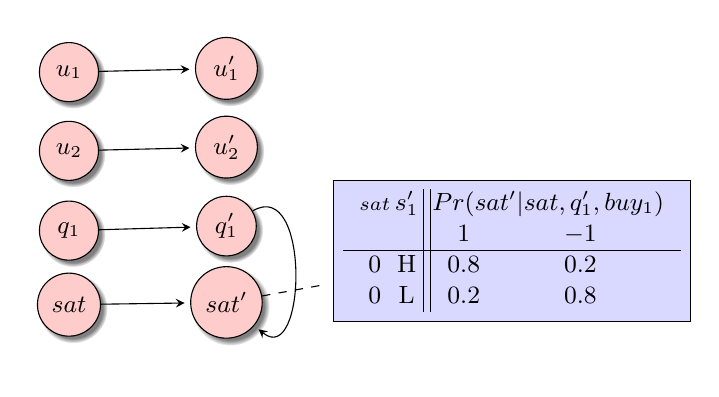
\begin{tikzpicture}[>=stealth,->,shorten >=2pt,looseness=.5,auto]
\matrix [matrix of math nodes,
column sep={20mm,between origins},
row sep={10mm,between origins},
nodes={circle, circular drop shadow, draw, minimum size=7.5mm, fill=red!20, font=\small}]
{
|(u_1)| u_1 & |(u'_1)| u'_1 \\
|(u_2)| u_2 & |(u'_2)| u'_2 \\
|(q_1)| q_1 & |(q'_1)|q'_1\\
|(sat)| sat & |(sat')| sat' \\
};
\node (some) at (4.6,-0.8) [draw, fill=blue!15,font=\small] {
\begin{tabular}{c@{\hspace{0.6mm}}c@{\hspace{0.6mm}}||c@{\hspace{0.6mm}}c@{\hspace{0.6mm}}}
     % \multicolumn{2}{c}{t}&\multicolumn{2}{c}{t+1}\\
     \centering
     \scriptsize
     \textbf{$sat$}&\textbf{$s'_1$}&\multicolumn{2}{@{\hspace{0.2mm}}c}{$Pr(sat'|sat,q'_1,buy_1)$}\\
     && \textbf{$1$} & \textbf{$-1$}\\
    \hline
     0 &H & 0.8 & 0.2 \\
    0&L & 0.2 & 0.8 \\
    \end{tabular}
    \hspace{-1mm}
};
\begin{scope}[every node/.style={font=\small\itshape}]
\draw (u_1)--(u'_1);
\draw (u_2)--(u'_2);
\draw (q_1)--(q'_1);
\draw (sat)--(sat');
\draw (q'_1)to [bend left, relative, out=120, in=50, looseness=1.5](sat');
\draw [-,dashed](sat')--(some);
%\draw (D) to [bend right, looseness=1]
%node [near start] {b} node [near end] {e} (A);
\end{scope}
\end{tikzpicture}
\vspace{-6mm}
\caption{DBN for $buy_{1}$} \label{fig:BuyS1}
\end{figure}
\vspace{-1mm}
 \begin{equation}
\begin{split}
\Pr(s'|s,buy_{1}) & = \Pr(u'_1,u'_2, q'_1,sat'|u_1,u_2,q_1,sat,buy_{1}) \\
& =  \Pr(u'_1|u_1,buy_{1})\times \Pr(u'_2|u_2,buy_{1}) \times \\
& \hspace{3.5mm}\Pr(q'_1|q_1,buy_{1}) \hspace{-0.5mm}\times\Pr(sat'|sat,q'_1,buy_{1})
\end{split}
 \label{eq:buy}
\end{equation}
 \textbf{Seller Query} Fig~\ref{fig:AskA1S1} shows the DBN and CPT for the action $seller\_query_{11} (sq_{11})$ (query $a_1$ about $s_1$).  Eqn~\ref{eq:sellerquery} shows that observing the quality of a seller $s_1$ through $o'$ is conditionally dependant on the current quality of the seller $q'_1$ (after the $seller\_query_{11}$ action) and the quality of the advisor $u'_1$, who provides opinion. $2$ possible observations are considered: $good$ (i.e., the advisor says that the seller is high quality) denoted by \textit{g} and $bad$ (the seller is said to be low quality) denoted by \textit{b}.  The observation probabilities for the $seller\_query_{ij}$ action are such that asking a trustworthy (T) advisor gives more accurate observations, while untrustworthy ones may provide a random (U) opinion or they can be adversarial (A) in nature.  We will obtain a similar figure for $seller\_query_{21}$ action.\\
  \begin{figure}[h!]
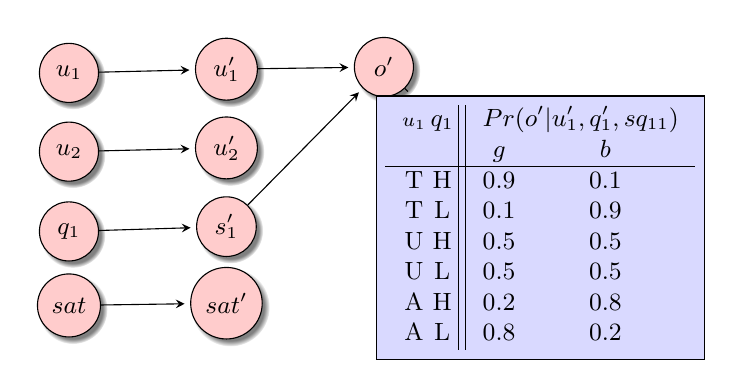
\begin{tikzpicture}[>=stealth,->,shorten >=2pt,looseness=.5,auto]
\matrix [matrix of math nodes,
column sep={20mm,between origins},
row sep={10mm,between origins},
nodes={circle, circular drop shadow, draw, minimum size=7.5mm, fill=red!20, font=\small}]
{
|(u_1)| u_1 & |(u'_1)| u'_1  &|(o')| o'\\
|(u_2)| u_2 & |(u'_2)| u'_2 \\
|(q_1)| q_1 & |(q'_1)| s'_1\\
|(sat)| sat & |(sat')| sat' \\
};
\node (some) at (4,-0.5) [draw, fill=blue!15,font=\small] {
\begin{tabular}{c@{\hspace{0.6mm}}c@{\hspace{0.6mm}}||c@{\hspace{0.6mm}}c@{\hspace{0.6mm}}}
     % \multicolumn{2}{c}{t}&\multicolumn{2}{c}{t+1}\\
     \centering
     \scriptsize
       \textbf{$u_1$}& \textbf{$q_1$} &\multicolumn{2}{c}{$Pr(o'|u_1',q_1',sq_{11})$}\\
     && \textbf{$g$} & \textbf{$b$}\\
      \hline
     T &H & 0.9 & 0.1 \\
     T&L & 0.1 & 0.9 \\
     U &H & 0.5 & 0.5 \\
     U & L & 0.5 & 0.5\\
     A &H & 0.2 & 0.8\\
     A & L & 0.8 & 0.2\\
    \end{tabular}
};
\begin{scope}[every node/.style={font=\small\itshape}]
\draw (u_1)--(u'_1);
\draw (u_2)--(u'_2);
\draw (q_1)--(q'_1);
\draw (sat)--(sat');
\draw (q'_1)--(o');
\draw (u'_1)--(o');
\draw [-,dashed](o')--(some);
%\draw (D) to [bend right, looseness=1]
%node [near start] {b} node [near end] {e} (A);
\end{scope}
\end{tikzpicture}
\vspace{-2mm}
\caption{DBN for $seller\_query_{11}$} \label{fig:AskA1S1}
\end{figure}
 \vspace{-3mm}
 \begin{figure}[h!]
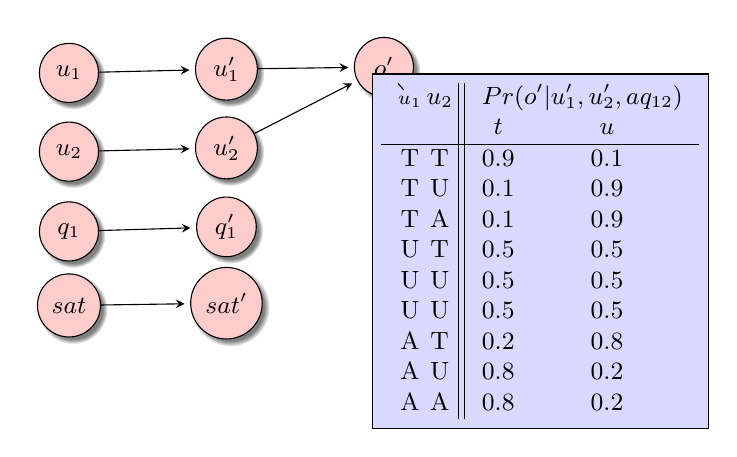
\begin{tikzpicture}[>=stealth,->,shorten >=2pt,looseness=.5,auto]
\matrix [matrix of math nodes,
column sep={20mm,between origins},
row sep={10mm,between origins},
nodes={circle, circular drop shadow, draw, minimum size=7.5mm, fill=red!20, font=\small}]
{
|(u_1)| u_1 & |(u'_1)| u'_1  &|(o')| o'\\
|(u_2)| u_2 & |(u'_2)| u'_2 \\
|(q_1)| q_1 & |(q'_1)| q'_1\\
|(sat)| sat & |(sat')| sat' \\
};
\node (some) at (4,-0.8) [draw, fill=blue!15,font=\small] {
\begin{tabular}{c@{\hspace{0.6mm}}c@{\hspace{0.6mm}}||c@{\hspace{0.6mm}}c@{\hspace{0.6mm}}}
     % \multicolumn{2}{c}{t}&\multicolumn{2}{c}{t+1}\\
     \centering
     \scriptsize
       \textbf{$u_1$}& \textbf{$u_2$} &\multicolumn{2}{c}{$Pr(o'|u_1',u_2',aq_{12})$}\\
     && \textbf{$t$} & \textbf{$u$}\\
      \hline
     T &T & 0.9 & 0.1 \\
     T&U & 0.1 & 0.9 \\
     T&A & 0.1 & 0.9 \\
      U&T & 0.5 & 0.5 \\
     U & U & 0.5 & 0.5\\
      U & U & 0.5 & 0.5\\
     A &T & 0.2 & 0.8 \\
     A & U & 0.8 & 0.2\\
      A & A & 0.8 & 0.2\\
    \end{tabular}
};
\begin{scope}[every node/.style={font=\small\itshape}]
\draw (u_1)--(u'_1);
\draw (u_2)--(u'_2);
\draw (q_1)--(q'_1);
\draw (sat)--(sat');
\draw (u'_1)--(o');
\draw (u'_2)--(o');
\draw [-,dashed](o')--(some);
%\draw (D) to [bend right, looseness=1]
%node [near start] {b} node [near end] {e} (A);
\end{scope}
\end{tikzpicture}
\vspace{-2mm}
\caption{DBN for $advisor\_query_{12}$} \label{fig:AskA1A2}
\end{figure}
 \begin{equation}
 \centering
\begin{split}
\Pr(o'|s,sq_{11})& =\Pr(o'|u_1',u_2',q_1',sat',sq_{11})\\
& =\Pr(o'|u_1',q_1',sq_{11})
\end{split}
 \label{eq:sellerquery}
\end{equation}
\textbf{Advisor Query} Fig~\ref{fig:AskA1A2} shows the DBN and CPT for the action $advisor\_query_{12} (aq_{12})$ (query $a_1$ about $a_2$).  Eqn~\ref{eq:advisorquery} show that observing the quality of advisor $a_2$ using the variable $o'$ (we use the same observation variable for simplicity) is conditionally dependant on the current quality of the advisor $u'_2$ (after the $advisor\_query_{12}$ action) and the quality of the advisor $a_1$ ($u'_1$), who provides opinion. We will obtain a similar figure for $advisor\_query_{21}$ action.
\begin{equation}
\begin{split}
\Pr(o'|s,aq_{12})&=\Pr(o'|u_1',u_2',s_1',sat',aq_{12})\\
&=\Pr(o'|u_1',u_2',aq_{12})
\end{split}
 \label{eq:advisorquery}
\end{equation}
The conditional probability tables in the above figures can be further compressed by exploiting context-specific independence which refers to the fact that some random variables are independent of each other in some contexts (i.e., for some specific values of other random variables). In general, context-specific independence allows one to compactly represent probability tables using decision trees (DTs) or algebraic decision diagrams (ADDs)~\cite{boutilier1996context}. We will show one such ADD for the CPT in Fig~\ref{fig:AskA1S1}.
 \begin{figure}[h!]
 \hspace{1mm}
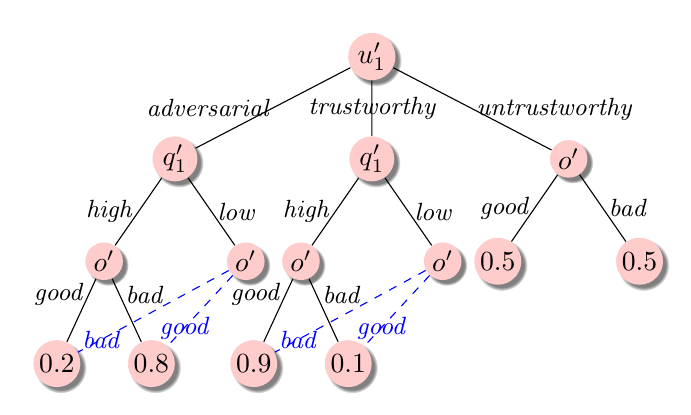
\begin{tikzpicture}
[level distance=13mm,
every node/.style={fill=red!20,circle,inner sep=1pt},
level 1/.style={sibling distance=25mm,nodes={fill=red!20}},
level 2/.style={sibling distance=18mm,nodes={fill=red!20}},
level 3/.style={sibling distance=12mm,nodes={fill=red!20}}]
\node [circular drop shadow] {$u'_1$}
child {node (AS) [circular drop shadow] {$q'_1$}
child {node (AOH) [circular drop shadow] {$o'$}
child {node (AHG)[circular drop shadow]{$0.2$}
edge from parent
node[pos=0.25,left,draw=none,fill=none,font=\small\itshape] {good}
}
child {node (AHL)[circular drop shadow]{$0.8$}
edge from parent
node[pos=0.25,right,draw=none,fill=none,font=\small\itshape] {bad}
}
edge from parent
node[left,draw=none,fill=none,font=\small\itshape] {high}
}
child {node (ATOL) [circular drop shadow] {$o'$}
edge from parent
node[right,draw=none,fill=none,font=\small\itshape] {low}
}
edge from parent
node[left,draw=none,fill=none,font=\small\itshape] {adversarial}
}
child {node (TS) [circular drop shadow] {$q'_1$}
child {node (TOH) [circular drop shadow] {$o'$}
child {node (HG)[circular drop shadow]{$0.9$}
edge from parent
node[pos=0.25,left,draw=none,fill=none,font=\small\itshape] {good}
}
child {node (HL)[circular drop shadow]{$0.1$}
edge from parent
node[pos=0.25,right,draw=none,fill=none,font=\small\itshape] {bad}
}
edge from parent
node[left,draw=none,fill=none,font=\small\itshape] {high}
}
child {node (TOL) [circular drop shadow] {$o'$}
edge from parent
node[right,draw=none,fill=none,font=\small\itshape] {low}
}
edge from parent
node[midway,draw=none,fill=none,font=\small\itshape] {trustworthy}
}
child {node [circular drop shadow] {$o'$}
child {node [circular drop shadow] {$0.5$}
edge from parent
node[left,draw=none,fill=none,font=\small\itshape] {good}
}
child {node [circular drop shadow] {$0.5$}
edge from parent
node[right,draw=none,fill=none,font=\small\itshape] {bad}
}
edge from parent
node[right,draw=none,fill=none,font=\small\itshape] {untrustworthy}
};
\draw (TOL)[-,dashed,blue] -- node [draw=none,fill=none,pos=0.85,font=\small\itshape] {bad}(HG);
\draw (TOL)[-,dashed,blue]-- node [draw=none,fill=none,pos=0.75,font=\small\itshape] {good}(HL);
\draw (ATOL)[-,dashed,blue]-- node [draw=none,fill=none,pos=0.75,font=\small\itshape] {good}(AHL);
\draw (ATOL)[-,dashed,blue]-- node [draw=none,fill=none,pos=0.85,font=\small\itshape] {bad}(AHG);
%\draw[dashed,->] (left node) -- (right node);
\end{tikzpicture}
\caption{ADD for $seller\_query_{11}$} \label{fig:ADDAskA1S1}
\end{figure}
\\ Fig.~\ref{fig:ADDAskA1S1} illustrates the ADD representations of the CPT for the observation variable $o'$ in Fig~\ref{fig:AskA1S1}. The value of $o'$ for some trust assignment for variables $u'_1, q'_1$ can be found by following the corresponding branch in the ADD.  Note that when $u'_1$ is $adversarial$ or $trustworthy$ in nature and seller quality $q'_1$ is $low$, $o'$ will result in the exact compliment of the values obtained when traversed through the path when $q'_1$ is $high$. This can be compactly represented, as shown using the blue dashed lines in Fig.~\ref{fig:ADDAskA1S1}. Also, when the advisor behaves in a random manner $u'_1 = untrustworthy$, $o'$ is independent of $q'_1$  and results in a value of $0.5$ whether $q'_1$ is of $high$ or $low$ quality. Hence, by using the notion of context-specific independence, the ADD in Fig.~\ref{fig:ADDAskA1S1} can encode with only $6$ leaves the $12$ values of the CPT in Fig~\ref{fig:AskA1S1}.  Thus we show how \SALEP{} exhibits conditional-independence and context-specific independence, which can be exploited by solvers such as Symbolic Perseus to find the optimal policy, especially for POMDPs with a large number of states.

\subsection{Belief Update in \SALEP{}}\label{sec:4}
The belief updates are performed such that they correlate the state factors in meaningful ways. For instance, observing $good$ after $seller\_query_{ij}$ should give more weights to states where the seller is $high$ quality $q_j = H$ and the advisor is $trustworthy$ $u_i = T$, and less weights to states where the seller is low quality $q_j = L$ and the advisor is $untrustworthy$ or $adversarial$ $u_i = U/A$.  Similarly, observing $T$ after $advisor\_query_{ii'}$ should put more weight on states where $u_i' = T$ and $u_i = T$, and decrease weight on states where $u_i' = U/A$ and $u_i = T$.

Fig.~\ref{fig:beleif} shows the partial \SALEP{} policy for the $1$ seller, $2$ advisors case. The transition and observation probabilities are same as those in Sec.~\ref{sec:factored}. As mentioned in Sec.~\ref{sec:factored}, each state $s=\left\langle \left\langle q_1\right\rangle, \left\langle u_1, u_2\right\rangle, sat\right\rangle$. The beliefs corresponding to each action (represented by nodes) are shown using tables associated with the nodes. The beliefs in  Fig.~\ref{fig:beleif} are presented in their factored form.  $AQ_{12}$ represents $advisor\_query_{12}$ and $SQ_{11}$ represents $seller\_query_{11}$. We have not shown the belief update for the variable $sat$ in the tables for simplicity.

Initially (before action $AQ_{12}$), the beliefs for advisors $u_1$ and $u_2$ are $0.5$ $trustworthy$ and $0.5$ $adversarial$ (we consider the attacking behavior to be $adversarial$) and those for seller $q_1$ is $0.5$ $high$ and $0.5$ $low$. When the agent receives an observation $o'=T$ after taking action $AQ_{12}$  (traversing through the left child of the root of the tree), the beliefs for $u_2$ is updated to \{$T=0.55$;$A=0.45$\}. Similarly the beliefs for $u_1$ is updated (after multiple $AQ_{21}$ actions), resulting in \{$T=0.61$;$A=0.38$\} for both $u_1$ and $u_2$. Advisors $u_1$ is determined to be $trustworthy$ and thereby queried about the seller (action $SQ_{11}$). When the agent receives an observation $o'=G (good)$, the beliefs for the seller are updated and thereby $BUY$ ($buy_1$) action is taken. Similarly, if the agent receives an observation $o'=B (bad)$, the $DNB$ ($do\_not\_buy$) action is taken. The beliefs obtained when the observation of $AQ_{12}$ action, $o'=U$ can be seen by traversing through the right child of the root.
 \begin{figure}[h!]
\hspace{1mm}
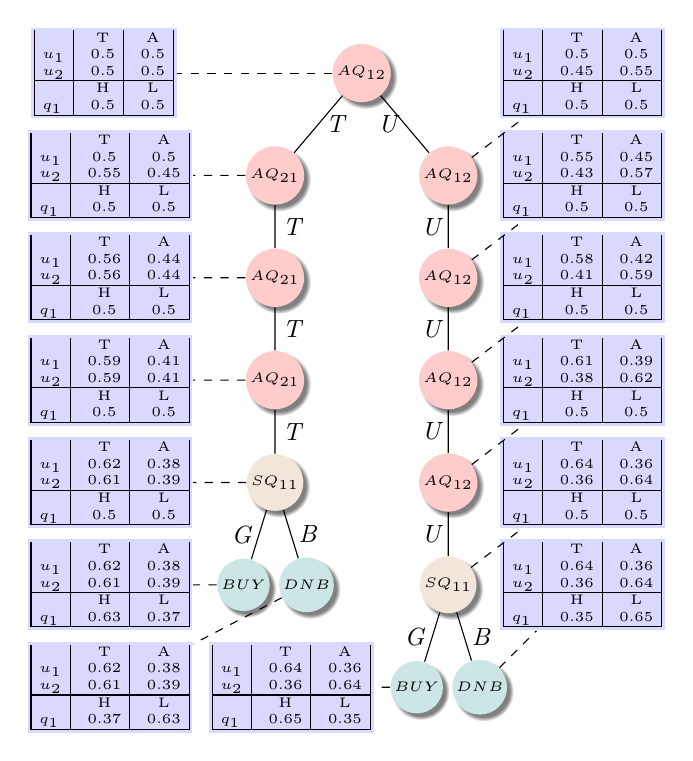
\begin{tikzpicture}
[level distance=13mm,
every node/.style={fill=red!20,circle,inner sep=1pt},
level 1/.style={sibling distance=22mm,nodes={fill=red!20}},
level 2/.style={sibling distance=18mm,nodes={fill=red!20}},
level 3/.style={sibling distance=12mm,nodes={fill=red!20}},
level 4/.style={sibling distance=8mm},
level 5/.style={sibling distance=8mm}
]
\node (root)[circular drop shadow,font=\tiny] {$AQ_{12}$}
child {node (T1)[circular drop shadow,font=\tiny] {$AQ_{21}$}
child {node (T2)[circular drop shadow,font=\tiny]{$AQ_{21}$}
child {node (T3)[circular drop shadow,font=\tiny]{$AQ_{21}$}
child {node (H4)[circular drop shadow,font=\tiny,fill={brown!20}]{$SQ_{11}$}
child {node (G5)[circular drop shadow,font=\tiny,fill={teal!20}]{$BUY$}
edge from parent
node[pos=0.50,left,draw=none,fill=none,font=\small\itshape] {G}
}
child {node (B5)[circular drop shadow,font=\tiny,fill={teal!20}]{$DNB$}
edge from parent
node[pos=0.50,right,draw=none,fill=none,font=\small\itshape] {B}
}
edge from parent
node[draw=none,right,fill=none,font=\small\itshape] {T}
}
edge from parent
node[pos=0.50,right,draw=none,fill=none,font=\small\itshape] {T}
}
edge from parent
node[pos=0.50,right,draw=none,fill=none,font=\small\itshape] {T}
}
edge from parent
node[pos=0.50,right,draw=none,fill=none,font=\small\itshape] {T}
}
child {node (A1)[circular drop shadow,font=\tiny]{$AQ_{12}$}
child {node (A2)[circular drop shadow,font=\tiny]{$AQ_{12}$}
child {node (A3)[circular drop shadow,font=\tiny]{$AQ_{12}$}
child {node (A4)[circular drop shadow,font=\tiny]{$AQ_{12}$}
child {node (HA5)[circular drop shadow,font=\tiny,fill={brown!20}]{$SQ_{11}$}
child {node (GA6)[circular drop shadow,font=\tiny,fill={teal!20}]{$BUY$}
edge from parent
node[pos=0.50,left,draw=none,fill=none,font=\small\itshape] {G}
}
child {node (BA6)[circular drop shadow,font=\tiny,fill={teal!20}]{$DNB$}
edge from parent
node[pos=0.50,right,draw=none,fill=none,font=\small\itshape] {B}
}
edge from parent
node[pos=0.50,left,draw=none,fill=none,font=\small\itshape] {U}
}
edge from parent
node[pos=0.50,left,draw=none,fill=none,font=\small\itshape] {U}
}
edge from parent
node[pos=0.50,left,draw=none,fill=none,font=\small\itshape] {U}
}
edge from parent
node[pos=0.50,left,draw=none,fill=none,font=\small\itshape] {U}
}
edge from parent
node[pos=0.50,left,draw=none,fill=none,font=\small\itshape] {U}
};
\node (roott) at (-2.2,0) [rectangle, left=4pt,fill=blue!15,font=\tiny] {
\begin{tabular}{|@{\hspace{1mm}}l@{\hspace{1mm}}|c@{\hspace{1mm}}|c@{\hspace{1mm}}|}
     \centering
     \scriptsize
   &T&A\\
     $u_1$ &0.5 & 0.5 \\
     $u_2$& 0.5 & 0.5 \\
       \hline
     &H&L\\
     $q_1$& 0.5 & 0.5 \\
     \hline
    \end{tabular}
};
\node (T1t) at (-2,-1.3) [rectangle, left =4pt, fill=blue!15,font=\tiny] {
\begin{tabular}{|@{\hspace{1mm}}l@{\hspace{1mm}}|c@{\hspace{1mm}}|c@{\hspace{1mm}}|}
     \centering
     \scriptsize
   &T&A\\
     $u_1$ &0.5 & 0.5 \\
     $u_2$& 0.55 & 0.45 \\
       \hline
     &H&L\\
     $q_1$& 0.5 & 0.5 \\
     \hline
    \end{tabular}
};
\node (T2t) at (-2,-2.6) [rectangle, left =4pt, fill=blue!15,font=\tiny] {
\begin{tabular}{|@{\hspace{1mm}}l@{\hspace{1mm}}|c@{\hspace{1mm}}|c@{\hspace{1mm}}|}
     \centering
     \scriptsize
   &T&A\\
     $u_1$ &0.56 & 0.44 \\
     $u_2$& 0.56& 0.44 \\
       \hline
     &H&L\\
     $q_1$& 0.5 & 0.5 \\
     \hline
    \end{tabular}
};
\node (T3t)at (-2,-3.9) [rectangle, left =4pt, fill=blue!15,font=\tiny] {
\begin{tabular}{|@{\hspace{1mm}}l@{\hspace{1mm}}|c@{\hspace{1mm}}|c@{\hspace{1mm}}|}
     \centering
     \scriptsize
   &T&A\\
     $u_1$&0.59 & 0.41 \\
     $u_2$& 0.59 & 0.41 \\
       \hline
     &H&L\\
     $q_1$& 0.5 & 0.5 \\
     \hline
    \end{tabular}
};
\node (H4t)at (-2,-5.2)[rectangle, left =4pt, fill=blue!15,font=\tiny] {
\begin{tabular}{|@{\hspace{1mm}}l@{\hspace{1mm}}|c@{\hspace{1mm}}|c@{\hspace{1mm}}|}
     \centering
     \scriptsize
   &T&A\\
     $u_1$&0.62 & 0.38 \\
     $u_2$& 0.61 & 0.39 \\
       \hline
     &H&L\\
     $q_1$& 0.5 & 0.5 \\
     \hline
    \end{tabular}
};
\node (G5t)at (-2,-6.5)[rectangle, left =4pt, fill=blue!15,font=\tiny] {
\begin{tabular}{|@{\hspace{1mm}}l@{\hspace{1mm}}|c@{\hspace{1mm}}|c@{\hspace{1mm}}|}
     \centering
     \scriptsize
   &T&A\\
    $u_1$&0.62 & 0.38 \\
     $u_2$& 0.61 & 0.39 \\
       \hline
     &H&L\\
     $q_1$& 0.63 & 0.37 \\
     \hline
    \end{tabular}
};
\node (B5t) at (-2,-7.8) [rectangle, left =4pt, fill=blue!15,font=\tiny] {
\begin{tabular}{|@{\hspace{1mm}}l@{\hspace{1mm}}|c@{\hspace{1mm}}|c@{\hspace{1mm}}|}
     \centering
     \scriptsize
   &T&A\\
     $u_1$&0.62 & 0.38 \\
     $u_2$& 0.61 & 0.39 \\
       \hline
     &H&L\\
     $q_1$& 0.37 & 0.63 \\
     \hline
    \end{tabular}
};
\node (A1t) at (4,0) [rectangle, left =4pt, fill=blue!15,font=\tiny] {
\begin{tabular}{|@{\hspace{1mm}}l@{\hspace{1mm}}|c@{\hspace{1mm}}|c@{\hspace{1mm}}|}
     \centering
     \scriptsize
   &T&A\\
     $u_1$&0.5 & 0.5 \\
     $u_2$& 0.45 & 0.55 \\
       \hline
     &H&L\\
     $q_1$& 0.5 & 0.5 \\
     \hline
    \end{tabular}
};
\node (A2t) at (4,-1.3) [rectangle, left =4pt, fill=blue!15,font=\tiny] {
\begin{tabular}{|@{\hspace{1mm}}l@{\hspace{1mm}}|c@{\hspace{1mm}}|c@{\hspace{1mm}}|}
     \centering
     \scriptsize
   &T&A\\
     $u_1$&0.55 & 0.45 \\
     $u_2$& 0.43& 0.57 \\
       \hline
     &H&L\\
     $q_1$& 0.5 & 0.5 \\
     \hline
    \end{tabular}
};
\node (A3t) at (4,-2.6) [rectangle, left =4pt, fill=blue!15,font=\tiny] {
\begin{tabular}{|@{\hspace{1mm}}l@{\hspace{1mm}}|c@{\hspace{1mm}}|c@{\hspace{1mm}}|}
     \centering
     \scriptsize
   &T&A\\
     $u_1$&0.58 & 0.42 \\
     $u_2$& 0.41 & 0.59 \\
       \hline
     &H&L\\
     $q_1$& 0.5 & 0.5 \\
     \hline
    \end{tabular}
};
\node (A4t) at (4,-3.9) [rectangle, left =4pt, fill=blue!15,font=\tiny] {
\begin{tabular}{|@{\hspace{1mm}}l@{\hspace{1mm}}|c@{\hspace{1mm}}|c@{\hspace{1mm}}|}
     \centering
     \scriptsize
   &T&A\\
     $u_1$&0.61 & 0.39 \\
     $u_2$& 0.38 & 0.62 \\
       \hline
     &H&L\\
     $q_1$& 0.5 & 0.5 \\
     \hline
    \end{tabular}
};
\node (HA5t) at (4,-5.2)[rectangle, left =4pt, fill=blue!15,font=\tiny] {
\begin{tabular}{|@{\hspace{1mm}}l@{\hspace{1mm}}|c@{\hspace{1mm}}|c@{\hspace{1mm}}|}
     \centering
     \scriptsize
   &T&A\\
     $u_1$&0.64 & 0.36 \\
     $u_2$& 0.36 & 0.64 \\
       \hline
     &H&L\\
     $q_1$& 0.5 & 0.5 \\
     \hline
    \end{tabular}
};
\node (GA6t) at (0.3,-7.8)[rectangle, left =4pt, fill=blue!15,font=\tiny] {
\begin{tabular}{|@{\hspace{1mm}}l@{\hspace{1mm}}|c@{\hspace{1mm}}|c@{\hspace{1mm}}|}
     \centering
     \scriptsize
   &T&A\\
       $u_1$&0.64 & 0.36 \\
     $u_2$& 0.36 & 0.64 \\
       \hline
     &H&L\\
     $q_1$& 0.65 & 0.35 \\
     \hline
    \end{tabular}
};
\node (BA6t) at (4,-6.5) [rectangle, left =4pt, fill=blue!15,font=\tiny] {
\begin{tabular}{|@{\hspace{1mm}}l@{\hspace{1mm}}|c@{\hspace{1mm}}|c@{\hspace{1mm}}|}
     \centering
     \scriptsize
   &T&A\\
       $u_1$&0.64 & 0.36 \\
     $u_2$& 0.36 & 0.64 \\
       \hline
     &H&L\\
    $q_1$& 0.35 & 0.65 \\
     \hline
    \end{tabular}
};
\begin{scope}[every node/.style={font=\small\itshape}]
\draw [-,dashed](root)--(roott);
\draw [-,dashed](T1)--(T1t);
\draw [-,dashed](T2)--(T2t);
\draw [-,dashed](T3)--(T3t);
\draw [-,dashed](H4)--(H4t);
\draw [-,dashed](G5)--(G5t);
\draw [-,dashed](B5)--(B5t);
\draw [-,dashed](A1)--(A1t);
\draw [-,dashed](A2)--(A2t);
\draw [-,dashed](A3)--(A3t);
\draw [-,dashed](A4)--(A4t);
\draw [-,dashed](HA5)--(HA5t);
\draw [-,dashed](GA6)--(GA6t);
\draw [-,dashed](BA6)--(BA6t);
\end{scope}
\end{tikzpicture}
\caption{(Partial) \SALEP{} Policy} \label{fig:beleif}
\vspace{-5mm}
\end{figure}



\section{Evaluation}\label{sec:5}
Detailed experiments are conducted to: 1) determine the efficiency of \SALEP{} in optimally choosing the right seller, in comparison with the other trust models and 2) analyze the scalability of \SALEP{}.

\subsection{Comparison with Other Trust Models}
  We evaluate the \SALEP{} model using the Agent Reputation and Trust (ART) testbed~\cite{fullam2005specification}. In the ART testbed, agents function as painting appraisers with varying levels of expertise in different artistic eras. Clients request appraisals for paintings from different eras; if an appraising agent does not have the expertise to complete the appraisal, it can request opinions from other appraiser agents (at a specified cost). Appraisers receive more clients, and thus more profit, for producing more accurate appraisals. The appraiser send the received opinions along with the weights (trustworthiness) of opinion providers to the simulation engine, which calculates the final value of the painting.

  To model the seller selection problem in a more effective way, we modify the ART testbed such that, appraisers receive more clients, and thus more profit for correctly identifying the quality of a painting (high/low), rather than accurately determining the value of the painting. Also, appraisers (irrespective of their level of expertise) can request opinions from other appraisers, about the appraisal and reputation of other appraisers. In the modified version, the appraisers are allowed to calculate the final appraisal of the painting, making the ART testbed decentralized. Modifying ART testbed in the above manner, makes it ideal to depict the seller selection problem, where the winning appraiser is assessed based on his bank balance in the long run.

  The specification of the ART testbed used for experimentation are:  1) client fee of $100$; 2) certainty cost $1$; 3) opinion cost $10$; 4) reputation cost $1$ and 5) Old Client Share Influence $0.1$. Using the above settings, we compare the performance of \SALEP{} with state-of-the-art trust models \textit{Advisor} POMDP, TRAVOS, Personalized and BLADE, each of which is modeled as an appraiser in the ART testbed. The trust models are assumed to behave honestly all the time, providing accurate opinions. Opinions refer to the quality of paintings (high/low) and reputation [$0-1$] of other appraisers.  Two attacking behaviors are considered: 1) random, where the appraisers provide opinion about the painting/other appraisers in a random manner; 2) adversarial, where the advisors provide the exact compliment of the true quality of the painting/other appraisers. The attackers are appraisers following the BRS model.
  \begin{filecontents}{advmulminaccuracy.dat}
1,95.0,90.0,100.0,60.0,100.0,
2,95.0,90.0,100.0,63.0,100.0,
3,97.5,95.0,100.0,63.5,100.0,
4,98.0,96.0,100.0,63.5,100.0,
5,98.5,97.0,100.0,64.0,100.0,
6,99.0,98.0,100.0,64.0,100.0,
7,99.0,98.0,100.0,64.5,100.0,
8,99.0,98.0,100.0,65.0,100.0,
9,99.0,98.0,100.0,66.0,100.0,
10,99.0,98.0,100.0,65.5,100.0,
11,99.0,98.0,100.0,65.5,100.0,
\end{filecontents}
\begin{filecontents}{advmulminbalance.dat}
1,940.5,381.5,381.5,943.5,386.5,
2,1619.5,422.0,1006.5,1036.5,996.5,
3,2476.0,780.5,1428.0,1642.0,1419.5,
4,3466.0,1220.5,1888.0,2132.0,1879.5,
5,4366.0,1621.0,2289.0,2538.0,2280.5,
6,5356.0,2061.0,2729.0,2928.0,2720.5,
7,6436.0,2541.0,3209.0,3218.0,3200.5,
8,7336.0,2982.0,3649.5,3666.5,3640.5,
9,8281.0,3402.0,4070.0,4015.5,4061.0,
10,9226.5,3822.5,4490.0,4264.5,4481.0,
11,10376.5,4972.5,5640.0,4364.5,5631.0,
\end{filecontents}
\begin{filecontents}{randommulminaccuracy.dat}
1,90.0,90.0,100.0,76.0,100.0,
2,90.0,90.0,100.0,76.5,100.0,
3,95.0,95.0,100.0,76.0,100.0,
4,96.0,96.0,100.0,76.0,100.0,
5,97.0,96.25,100.0,77.0,100.0,
6,98.1,96.5,100.0,78.0,100.0,
7,98.2,97.0,100.0,76.5,100.0,
8,98.3,97.25,100.0,76.5,100.0,
9,98.4,97.5,100.0,76.0,100.0,
10,98.5,97.5,100.0,75.5,100.0,
11,98.5,97.5,100.0,75.5,100.0,
\end{filecontents}
\begin{filecontents}{randommulminbalance.dat}
1,943.5,382.5,381.0,944.5,381.5,
2,1041.5,430.5,1059.5,1041.5,1069.5,
3,1851.5,788.0,1500.5,1848.0,1511.0,
4,2841.5,1228.0,1980.5,2338.0,1991.0,
5,3743.0,1630.0,2382.0,2745.0,2386.0,
6,4868.0,1870.0,2882.0,3135.0,2886.0,
7,5948.0,2330.0,3362.0,3325.0,3366.0,
8,7028.5,2810.0,3842.0,3614.5,3846.0,
9,7929.0,3210.5,4243.0,3821.0,4247.0,
10,8919.0,3650.5,4683.0,3911.0,4687.0,
11,10119.0,4850.5,5883.0,4011.0,5887.0,
\end{filecontents}
\begin{filecontents}{advmulmaxaccuracy.dat}
1,95.0,90.0,90.0,40.0,80.0,
2,95.0,90.0,90.0,41.0,81.0,
3,97.5,95.0,95.0,41.0,90.0,
4,98.0,96.0,96.0,42.0,93.0,
5,98.5,97.0,97.0,42.5,95.0,
6,99.0,98.0,98.0,43.0,96.0,
7,99.0,98.0,98.0,43.5,96.0,
8,99.0,98.0,98.0,45.0,97.0,
9,99.0,98.0,98.0,45.0,97.0,
10,99.0,98.0,98.0,44.0,97.0,
11,99.0,98.0,98.0,44.0,97.0,
\end{filecontents}
\begin{filecontents}{advmulmaxbalance.dat}
1,840.0,81.0,81.0,974.0,81.0,
2,1612.5,98.5,98.5,1070.5,93.5,
3,2609.0,180.0,165.0,1166.0,200.0,
4,3509.5,280.5,266.0,1969.0,301.0,
5,4499.5,390.5,376.0,2458.5,411.0,
6,5489.5,501.5,486.0,2847.5,521.0,
7,6390.5,602.0,586.5,3252.0,621.5,
8,7380.5,712.0,697.5,3641.0,731.5,
9,8280.5,812.5,797.5,3849.0,831.5,
10,9270.5,922.5,907.5,3938.5,941.5,
11,10370.5,2022.5,2007.5,4038.5,2041.5,
\end{filecontents}
\begin{filecontents}{randommulmaxaccuracy.dat}
1,80.0,90.0,95.0,70.0,90.0,
2,86,91.5,96.0,69.0,93.5,
3,92.0,93,96.25,68.0,96.5,
4,95,94,96.5,68.5,97.5,
5,96.5,94.5,96.5,71.0,98.0,
6,97.5,95,96.5,71.5,98.5,
7,97.5,95.5,97.0,70.0,98.75,
8,98.0,96.0,97.25,69.5,99.0,
9,98.0,96.0,97.5,69.0,99.0,
10,98.0,96.0,97.5,68.5,99.0,
11,98.0,96.0,97.5,68.5,99.0,
\end{filecontents}
\begin{filecontents}{randommulmaxbalance.dat}
1,921.5,83.5,84.0,971.0,83.0,
2,1554.5,171.0,592.0,1486.0,170.5,
3,3399.5,232.0,793.0,1977.0,382.5,
4,5066.5,403.5,924.5,2367.5,569.5,
5,6508.0,515.0,1031.0,2762.5,730.0,
6,7993.0,615.0,1131.5,3297.0,900.0,
7,9613.0,740.0,1311.5,3834.5,1086.0,
8,10828.0,870.0,1446.5,4283.0,1221.0,
9,12133.0,1020.5,1526.5,4572.5,1376.0,
10,13798.5,1041.0,1626.5,4824.5,1561.5,
11,15298.5,2441.0,2376.5,4974.5,3161.5,
\end{filecontents}
\hspace{-4mm}
\begin{figure*}[!htbp]
\centering
\ref{named}\\
\tikzset{every mark/.append style={scale=1.2}}
\hspace{-4mm}
\begin{tikzpicture}[scale=0.82]
\pgfplotsset{title style={at={(0.5,-0.4)}}}
\begin{axis}[title= (a), legend columns=-1,small,width=6cm, enlarge y limits=false,grid=major,xlabel={Time Point},ylabel={Accuracy},ylabel style={yshift=-2em}, legend style={font=\tiny,mark size=2pt, /tikz/column 2/.style={column sep=5pt,},},legend entries={SALE,BLADE,Personalized,Advisor,TRAVOS},legend to name=named,xlabel style={yshift=0.6em}]
\addplot[mark=10-pointed star,red] table[x index=0,y index=1,col sep=comma] {advmulminaccuracy.dat};
\addplot[mark=triangle*,black]table[x index=0,y index=2,col sep=comma] {advmulminaccuracy.dat};
\addplot[mark=o,black] table[x index=0,y index=3,col sep=comma] {advmulminaccuracy.dat};
\addplot[mark=diamond*,black]  table[x index=0,y index=4,col sep=comma] {advmulminaccuracy.dat};
\addplot[mark=x,black] table[x index=0,y index=5,col sep=comma] {advmulminaccuracy.dat};
\end{axis}
\end{tikzpicture}
\hspace{-4mm}
\begin{tikzpicture}[scale=0.82]
\pgfplotsset{title style={at={(0.5,-0.4)}}}
\begin{axis}[title= (b),small,width=6cm,enlarge y limits=false,grid=major,xlabel={Time Point},ylabel={Bank Balance},ylabel style={yshift=-1.7em},xlabel style={yshift=0.6em}]
\addplot[mark=10-pointed star,red] table[x index=0,y index=1,col sep=comma] {advmulminbalance.dat};
\addplot[mark=triangle*,black]table[x index=0,y index=2,col sep=comma] {advmulminbalance.dat};
\addplot[mark=o,black] table[x index=0,y index=3,col sep=comma] {advmulminbalance.dat};
\addplot[mark=diamond*,black]  table[x index=0,y index=4,col sep=comma] {advmulminbalance.dat};
\addplot[mark=x,black] table[x index=0,y index=5,col sep=comma] {advmulminbalance.dat};
\end{axis}
\end{tikzpicture}
\hspace{-4mm}
\begin{tikzpicture}[scale=0.82]
\pgfplotsset{title style={at={(0.5,-0.4)}}}
\begin{axis}[title= (c),small,width=6cm,enlarge y limits=false,grid=major,xlabel={Time Point},ylabel={Accuracy},ylabel style={yshift=-2em},xlabel style={yshift=0.6em}]
\addplot[mark=10-pointed star,red] table[x index=0,y index=1,col sep=comma] {randommulminaccuracy.dat};
\addplot[mark=triangle*,black]table[x index=0,y index=2,col sep=comma] {randommulminaccuracy.dat};
\addplot[mark=o,black] table[x index=0,y index=3,col sep=comma] {randommulminaccuracy.dat};
\addplot[mark=diamond*,black]  table[x index=0,y index=4,col sep=comma] {randommulminaccuracy.dat};
\addplot[mark=x,black] table[x index=0,y index=5,col sep=comma] {randommulminaccuracy.dat};
\end{axis}
\end{tikzpicture}
\hspace{-4mm}
\begin{tikzpicture}[scale=0.82]
\pgfplotsset{title style={at={(0.5,-0.4)}}}
\begin{axis}[title= (d),small,width=6cm,enlarge y limits=false,grid=major,xlabel={Time Point},ylabel={Bank Balance},ylabel style={yshift=-1.7em},xlabel style={yshift=0.6em}]
\addplot[mark=10-pointed star,red] table[x index=0,y index=1,col sep=comma] {randommulminbalance.dat};
\addplot[mark=triangle*,black]table[x index=0,y index=2,col sep=comma] {randommulminbalance.dat};
\addplot[mark=o,black] table[x index=0,y index=3,col sep=comma] {randommulminbalance.dat};
\addplot[mark=diamond*,black]  table[x index=0,y index=4,col sep=comma] {randommulminbalance.dat};
\addplot[mark=x,black] table[x index=0,y index=5,col sep=comma] {randommulminbalance.dat};
\end{axis}
\end{tikzpicture} \\
\vspace{-3mm}
\hspace{-4mm}
\begin{tikzpicture}[scale=0.82]
\pgfplotsset{title style={at={(0.5,-0.4)}}}
\begin{axis}[title= (e),small,width=6cm,enlarge y limits=false,grid=major,xlabel={Time Point},ylabel={Accuracy},ylabel style={yshift=-2em},xlabel style={yshift=0.6em}]
\addplot[mark=10-pointed star,red] table[x index=0,y index=1,col sep=comma] {advmulmaxaccuracy.dat};
\addplot[mark=triangle*,black]table[x index=0,y index=2,col sep=comma] {advmulmaxaccuracy.dat};
\addplot[mark=o,black] table[x index=0,y index=3,col sep=comma] {advmulmaxaccuracy.dat};
\addplot[mark=diamond*,black]  table[x index=0,y index=4,col sep=comma] {advmulmaxaccuracy.dat};
\addplot[mark=x,black] table[x index=0,y index=5,col sep=comma] {advmulmaxaccuracy.dat};
\end{axis}
\end{tikzpicture}
\hspace{-4mm}
\begin{tikzpicture}[scale=0.82]
\pgfplotsset{title style={at={(0.5,-0.4)}}}
\begin{axis}[title= (f),small,width=6cm,enlarge y limits=false,grid=major,xlabel={Time Point},ylabel={Bank Balance},ylabel style={yshift=-1.7em},xlabel style={yshift=0.6em}]
\addplot[mark=10-pointed star,red] table[x index=0,y index=1,col sep=comma] {advmulmaxbalance.dat};
\addplot[mark=triangle*,black]table[x index=0,y index=2,col sep=comma] {advmulmaxbalance.dat};
\addplot[mark=o,black] table[x index=0,y index=3,col sep=comma] {advmulmaxbalance.dat};
\addplot[mark=diamond*,black]  table[x index=0,y index=4,col sep=comma] {advmulmaxbalance.dat};
\addplot[mark=x,black] table[x index=0,y index=5,col sep=comma] {advmulmaxbalance.dat};
\end{axis}
\end{tikzpicture}
\hspace{-4mm}
\begin{tikzpicture}[scale=0.82]
\pgfplotsset{title style={at={(0.5,-0.4)}}}
\begin{axis}[title= (g),small,width=6cm,enlarge y limits=false,grid=major,xlabel={Time Point},ylabel={Accuracy},ylabel style={yshift=-2em},xlabel style={yshift=0.6em}]
\addplot[mark=10-pointed star,red] table[x index=0,y index=1,col sep=comma] {randommulmaxaccuracy.dat};
\addplot[mark=triangle*,black]table[x index=0,y index=2,col sep=comma] {randommulmaxaccuracy.dat};
\addplot[mark=o,black] table[x index=0,y index=3,col sep=comma] {randommulmaxaccuracy.dat};
\addplot[mark=diamond*,black]  table[x index=0,y index=4,col sep=comma] {randommulmaxaccuracy.dat};
\addplot[mark=x,black] table[x index=0,y index=5,col sep=comma] {randommulmaxaccuracy.dat};
\end{axis}
\end{tikzpicture}
\hspace{-4mm}
\begin{tikzpicture}[scale=0.82]
\pgfplotsset{title style={at={(0.5,-0.4)}}}
\begin{axis}[title= (h),small,width=6cm,enlarge y limits=false,grid=major,xlabel={Time Point},ylabel={Bank Balance},ylabel style={yshift=-1.7em},xlabel style={yshift=0.6em}]
\addplot[mark=10-pointed star,red] table[x index=0,y index=1,col sep=comma] {randommulmaxbalance.dat};
\addplot[mark=triangle*,black]table[x index=0,y index=2,col sep=comma] {randommulmaxbalance.dat};
\addplot[mark=o,black] table[x index=0,y index=3,col sep=comma] {randommulmaxbalance.dat};
\addplot[mark=diamond*,black]  table[x index=0,y index=4,col sep=comma] {randommulmaxbalance.dat};
\addplot[mark=x,black] table[x index=0,y index=5,col sep=comma] {randommulmaxbalance.dat};
\end{axis}
\end{tikzpicture}
\vspace{-3mm}
\caption{Sequential Setting} \label{fig:Sequential}
\vspace{-3mm}
\end{figure*}

For \SALEP{}, the rewards are: $R(s,seller\_query_{ij})=10$, $R(s,advisor\_query_{ii'})=1$, $R_{sat}=100$, $R_{unsat}=-100$ and the penalty for taking the $do\_not\_buy$ action when in fact there is a seller of high enough quality is $-100$, otherwise the reward is $100$. In the experiments, we use Symbolic Perseus~\cite{poupart2005exploiting}, a state- of-the-art POMDP solver, which reads problems in a standardized POMDP description format. Symbolic Perseus exploits the \textit{factored} nature of  \SALEP{} and helps to achieve better scalability.

The evaluation metrics used are: 1) $accuracy$ which is the percentage of  appraisals, for which the quality of painting has been correctly identified by the appraiser (trust model); 2) bank balance, representing the profit gained by identifying the correct quality of paintings (in an optimal way).

We first conduct experiments in a sequential setting where appraisers are engaged in multiple transactions. The ART testbed simulation is run for $10$ timesteps and the average number of clients per appraiser is $10$. In \SALEP{}, each painting appraisal problem is modeled as a separate POMDP and the modified belief state resulting from advice in a previous problem is retained and is used as the initial belief for solving the next painting appraisal problem i;e (finding the quality of the next painting).

 Fig~\ref{fig:Sequential} shows the results in the sequential setting. From Fig~\ref{fig:Sequential}, we can find that accuracy and bank balance of most trust models increase with time, depicting that experience from previous transactions can significantly affect the performance of the trust models. Fig.\ref{fig:Sequential} (a-d) show the case when trustworthy appraisers form the majority in the market ($2$ untrustworthy appraisers are introduced) and  Fig.\ref{fig:Sequential} (e-h) show that case when attackers form the majority ($5$ attackers are introduced).

In Fig.\ref{fig:Sequential} (a-b), the attackers are $adversarial$ in nature.  From Fig.\ref{fig:Sequential} (a), we find that accuracy of \SALEP{} is $95.0$\% in the beginning. This is because \SALEP{}, at times cannot accurately determine the quality of paintings, in the presence of attackers who provide inaccurate opinions and when the appraiser has no prior experience in the market. However, its accuracy increases to $99.0$\%, at the end of simulation, as it uses previous transaction information to identify $adversarial$ appraisers and refrain from asking opinions. TRAVOS and Personalized obtain a better accuracy of $100$\% throughout the simulation. This is because the majority of the advisors (other appraisers) are trustworthy. TRAVOS and Personalized use the majority rule to determine the quality of the painting, when the appraiser has no experience in the market and they also incorporate the usage of history information, which helps to determine the quality of painting in the subsequent timesteps correctly. BLADE obtains an initial accuracy of $90.0$\%, as it cannot appropriately determine the quality of  painting when the appraiser is a new comer, since it mainly relies on previous experience with advisors to reinterpret their opinions. However, its accuracy increases with time due to the increase in number of transactions. \textit{Advisor} POMDP considers all appraisers to be trustworthy and hence its accuracy depends on the probability of choosing a trustworthy appraiser to ask opinion, thereby obtaining a low accuracy of  $65.5$\%.
%\begin{filecontents}{advsingleaccuracy.dat}
%0,80.0,0.0,100.0,100.0,100.0,
%1,30.0,0.0,100.0,50.0,100.0,
%2,40.0,0.0,100.0,50.0,100.0,
%3,40.0,0.0,100.0,50.0,100.0,
%4,0.0,0.0,0.0,50.0,0.0,
%5,0.0,0.0,0.0,50.0,0.0,
%\end{filecontents}
%\begin{filecontents}{advsinglebalance.dat}
%0,166.6,59.1,161.6,218.4,181.3,
%1,114.0,51.7,180.7,147.4,178.1,
%2,126.1,39.8,175.6,146.2,168.8,
%3,126.1,33.0,181.4,146.0,178.3,
%4,84.7,21.1,18.2,198.3,22.9,
%5,84.4,13.1,8.1,197.0,12.9,
%\end{filecontents}

\begin{filecontents}{advsingleaccuracy.dat}
0,100.0,0.0,100.0,100.0,100.0,
1,70.0,0.0,100.0,80.0,100.0,
2,60.0,0.0,100.0,70.0,100.0,
3,50.0,0.0,100.0,60.0,100.0,
4,40.0,0.0,0.0,50.0,0.0,
5,0.0,0.0,0.0,40.0,0.0,
\end{filecontents}
\begin{filecontents}{advsinglebalance.dat}
0,188.8,59.4,159.3,192.4,160.1,
1,160.3,48.1,169.5,174.1,168.3,
2,153.5,39.3,158.3,164.1,158.3,
3,145.6,31.0,148.3,155.7,148.5,
4,142.6,18.3,18.4,167.1,18.2,
5,91.0,8.1,8.0,177.0,8.0,
\end{filecontents}
\begin{filecontents}{randomsingleaccuracy.dat}
0,100.0,0.0,100.0,100.0,100.0,
1,100.0,0.0,100.0,90.0,100.0,
2,90.0,0.0,100.0,90.0,100.0,
3,80.0,0.0,100.0,70.0,100.0,
4,70.0,0.0,60.0,60.0,60.0,
5,50.0,0.0,60.0,60.0,60.0,
\end{filecontents}
\begin{filecontents}{randomsinglebalance.dat}
0,191.4,58.7,158.9,192.7,158.3,
1,192.4,48.8,148.4,183.8,148.1,
2,182.9,38.4,138.3,184.6,138.7,
3,172.6,28.6,128.3,165.7,128.0,
4,163.6,18.3,97.7,156.2,98.2,
5,142.6,8.2,68.4,157.7,68.2,
\end{filecontents}
%\begin{filecontents}{randomsingleaccuracy.dat}
%0,100.0,0.0,100.0,100.0,100.0,
%1,100.0,0.0,100.0,80.0,100.0,
%2,100.0,0.0,100.0,70.0,100.0,
%3,90.0,0.0,100.0,60.0,100.0,
%4,90.0,0.0,70.0,50.0,70.0,
%5,70.0,0.0,50.0,50.0,50.0,
%\end{filecontents}
%\begin{filecontents}{randomsinglebalance.dat}
%0,191.1,59.0,158.7,192.5,158.7,
%1,192.1,48.7,148.2,173.6,148.2,
%2,192.4,38.4,138.6,164.6,139.1,
%3,181.4,28.2,138.6,155.5,138.6,
%4,181.2,18.4,69.2,147.3,128.2,
%5,173.2,8.2,88.8,147.2,88.1,
%\end{filecontents}
\begin{filecontents}{datax.dat}
0,100,0,100,100,100,0
1,100,0,100,90,100,0
2,90,0,100,80,100,0
3,90,0,100,70,100,0
4,90,0,90,70,100,0
5,60,0,90,50,100,0
\end{filecontents}
\begin{figure*}[!htbp]
\centering
\ref{named}\\
\tikzset{every mark/.append style={scale=1.2}}
\hspace{-4mm}
\begin{tikzpicture}[scale=0.82]
\pgfplotsset{title style={at={(0.5,-0.5)}}}
\begin{axis}[title= (a),ymin=-10, ymax=110,legend columns=-1,small,width=6cm, enlarge y limits=false,grid=major,xlabel={No. of Attackers},ylabel={Accuracy},ylabel style={yshift=-2em}, legend style={font=\tiny,mark size=2pt, /tikz/column 2/.style={column sep=5pt,},},legend entries={SALE,BLADE,Personalized,Advisor,TRAVOS},legend to name=named,xlabel style={yshift=0.6em}]
\addplot[mark=10-pointed star,red] table[x index=0,y index=1,col sep=comma] {advsingleaccuracy.dat};
\addplot[mark=triangle*,black]table[x index=0,y index=2,col sep=comma] {advsingleaccuracy.dat};
\addplot[mark=o,black] table[x index=0,y index=3,col sep=comma] {advsingleaccuracy.dat};
\addplot[mark=diamond*,black]  table[x index=0,y index=4,col sep=comma] {advsingleaccuracy.dat};
\addplot[mark=x,black] table[x index=0,y index=5,col sep=comma] {advsingleaccuracy.dat};
\end{axis}
\end{tikzpicture}
\begin{tikzpicture}[scale=0.82]
\pgfplotsset{title style={at={(0.5,-0.5)}}}
\begin{axis}[title= (b),small,ymin=0, ymax=220,width=6cm,enlarge y limits=false,grid=major,xlabel={No. of Attackers},ylabel={Bank Balance},ylabel style={yshift=-1.7em},xlabel style={yshift=0.6em}]
\addplot[mark=10-pointed star,red] table[x index=0,y index=1,col sep=comma] {advsinglebalance.dat};
\addplot[mark=triangle*,black]table[x index=0,y index=2,col sep=comma] {advsinglebalance.dat};
\addplot[mark=o,black] table[x index=0,y index=3,col sep=comma] {advsinglebalance.dat};
\addplot[mark=diamond*,black]  table[x index=0,y index=4,col sep=comma] {advsinglebalance.dat};
\addplot[mark=x,black] table[x index=0,y index=5,col sep=comma] {advsinglebalance.dat};
\end{axis}
\end{tikzpicture}
\begin{tikzpicture}[scale=0.82]
\pgfplotsset{title style={at={(0.5,-0.5)}}}
\begin{axis}[title= (c),ymin=-10, ymax=110,small,width=6cm,enlarge y limits=false,grid=major,xlabel={No. of Attackers},ylabel={Accuracy},ylabel style={yshift=-2em},xlabel style={yshift=0.6em}]
\addplot[mark=10-pointed star,red] table[x index=0,y index=1,col sep=comma] {randomsingleaccuracy.dat};
\addplot[mark=triangle*,black]table[x index=0,y index=2,col sep=comma] {randomsingleaccuracy.dat};
\addplot[mark=o,black] table[x index=0,y index=3,col sep=comma] {randomsingleaccuracy.dat};
\addplot[mark=diamond*,black]  table[x index=0,y index=4,col sep=comma] {randomsingleaccuracy.dat};
\addplot[mark=x,black] table[x index=0,y index=5,col sep=comma] {randomsingleaccuracy.dat};
\end{axis}
\end{tikzpicture}
\begin{tikzpicture}[scale=0.82]
\pgfplotsset{title style={at={(0.5,-0.5)}}}
\begin{axis}[title= (d),small,ymin=0, ymax=220,width=6cm,enlarge y limits=false,grid=major,xlabel={No. of Attackers},ylabel={Bank Balance},ylabel style={yshift=-1.7em},xlabel style={yshift=0.6em}]
\addplot[mark=10-pointed star,red] table[x index=0,y index=1,col sep=comma] {randomsinglebalance.dat};
\addplot[mark=triangle*,black]table[x index=0,y index=2,col sep=comma] {randomsinglebalance.dat};
\addplot[mark=o,black] table[x index=0,y index=3,col sep=comma] {randomsinglebalance.dat};
\addplot[mark=diamond*,black]  table[x index=0,y index=4,col sep=comma] {randomsinglebalance.dat};
\addplot[mark=x,black] table[x index=0,y index=5,col sep=comma] {randomsinglebalance.dat};
\end{axis}
\end{tikzpicture}
\vspace{-3mm}
\caption{Single Transaction Setting} \label{fig:Single}
\vspace{-3mm}
\end{figure*}
Fig.\ref{fig:Sequential} (b) shows the bank balance of the appraisers corresponding to Fig.\ref{fig:Sequential} (a). We find that \SALEP{} obtains the highest bank balance. This is because \SALEP{} uses fewer opinion transactions (request opinion about paintings from other appraisers), the costs of which is $10$. \SALEP{} mainly relies on reputation transactions (request reputation about appraisers from other appraisers) with a cost of $1$, to determine a trustworthy appraiser and then request opinions about the paintings. TRAVOS, Personalized and BLADE, on the other hand simply query all appraisers about the quality of  the paintings resulting in a huge cost, when compared to the profit gained by accurately determining the quality of the painting. Also, TRAVOS and Personalized do not query about the reputation of other appraisers to determine their trustworthiness, which is an unique feature offered by the \SALEP{} model. Though \textit{Advisor} POMDP uses fewer opinion transactions, its bank balance is lower than \SALEP{} due to its lower accuracy.

In Fig.\ref{fig:Sequential} (c-d), the attackers are $random$ in nature. Fig.\ref{fig:Sequential} (c) shows that accuracy of  \SALEP{} increases from $90.0$\% to $98.5$\%. However, from Fig.\ref{fig:Sequential} (c), we can find that accuracy of \SALEP{} increases at a slower rate than in  Fig.\ref{fig:Sequential} (a). This is because the attackers are $random$ in nature, whereby they may also provide truthful opinions at times. \SALEP{} assumes consistent advisor behavior and hence requires more number of transactions to learn about the trustworthiness of the $random$ attackers than when they behave in an $adversarial$ manner, always providing incorrect opinions. TRAVOS and Personalized obtain an accuracy of $100$\% thought the simulation and accuracy of BLADE increases from $90.0$\% to $97.5$\%. The accuracy of \textit{Advisor} POMDP increases, then decreases. Such behavior is hugely attributed to the random nature of the advisor who provide opinions. Again \SALEP{} obtains a higher bank balance than others as shown in Fig.\ref{fig:Sequential} (d).

In Fig.\ref{fig:Sequential} (e-f), the attackers are $adversarial$ in nature and form the majority. Fig.\ref{fig:Sequential} (e) shows that \SALEP{} follows a similar trend as in Fig.\ref{fig:Sequential} (a). But, we find that TRAVOS and Personalized obtain an initial accuracy of $90.0$\% and $80.0$\% respectively when compared to $100$\% in Fig.\ref{fig:Sequential} (a). This is because when the appraiser is newcomer, both approaches rely on the majority rule and since the majority appraisers are attackers in this case, their accuracy is less. However, with experience their accuracy increases.  Again, Fig.\ref{fig:Sequential} (f) shows that \SALEP{} obtains a higher bank balance than others.

Fig.\ref{fig:Sequential} (g), (h) show the case when attackers are $random$ in nature and form the majority. The initial accuracy of  \SALEP{} is $80.0$\% (as compared to $90.0$\% in Fig.\ref{fig:Sequential} (c)), due to the increase in the number of attackers. Also TRAVOS outperforms Personalized as it is able to correctly identify the trustworthiness of the appraisers by comparing their opinions on paintings with similar value. Personalized considers all previous opinions from appraisers, thereby increasing the chance to incorrectly model the trustworthiness of the attackers due to their random behavior. The accuracy of the \textit{Advisor} POMDP is also lower than the case where the trustworthy appraisers form the majority.

We also conduct experiments to verify the performance of \SALEP{} in a single transaction setting.  Here all appraisers are new comers to the market and have no prior experience (which is the case with most real world e-market places). The simulation is run only for a single time step and average number of clients per agent is limited to $1$. Fig.~\ref{fig:Single} shows the results of the single transaction setting.  Fig.~\ref{fig:Single}(a-b) show the result when the attacking behavior is $adversarial$ in nature.  The accuracy of \SALEP{} decreases with the increase in the number of attackers, as the probability of obtaining an incorrect opinion increases with the increase in the number of attackers. TRAVOS and Personalized obtain a greater accuracy of 100\% for the cases when the majority of the advisors are honest in nature (No.of Attackers < $4$).  In the scenario with equal number of trustworthy and adversarial appraisers \SALEP{} performs better than TRAVOS and Personalized. The \textit{Advisor} POMDP considers all advisors to be trustworthy and relies on the opinion from the single appraiser whom it asks opinion. Its performance is hugely dependant on the honesty of the appraiser it chooses to ask opinion, thereby making its accuracy as the probability of selecting the honest appraiser as shown in Fig.~\ref{fig:Single} (a).  Fig.~\ref{fig:Single}(b) shows the bank balance of the trust models which correspond to the accuracy in Fig.~\ref{fig:Single}(a). We can see that \SALEP{} obtains a better bank balance then TRAVOS and Personalized even in a single transaction setting. The \textit{Advisor} POMDP achieves the best bank balance in all cases because, it performs fewer opinion transactions. However, its performance is hugely reliable on the single advisor it chooses to ask opinions, which cannot be successful at all times. Also,  its performance decreases in multiple transaction settings as shown in Fig.~\ref{fig:Sequential}.
  Fig.~\ref{fig:Single}(c), (d) show the results in a scenario when the attacking behavior is $random$. In general all trust models perform better than the $adversarial$ scenario, as the $random$ attackers can provide correct opinions in some cases.  Again from Fig.~\ref{fig:Single}(d), we find that \SALEP{} obtains a better bank balance than others.

\subsection{Scalability of \SALEP{}}  In \SALEP{},  the state of the environment within a POMDP is defined using a set of state variables. The state space of such a factored representation is exponential in the number of variables, due to which Algebraic Decision Diagram (ADDs) were introduced. In this section, we will discuss the scalability of \SALEP{}, utilizing the  Symbolic Perseus. Table~\ref{table:scalability} shows the time taken to generate the policy for the given number of sellers and advisors. The number of state variables in each case is also shown. For the case with $2$ advisors and $3$ sellers, the time taken is $18.89$s  and $22.48$s when the attackers are $adversarial$ and $random$ respectively. We can see that, to solve for the case with $4$ sellers and $8$ advisors, the time taken is nearly $3$ hours, when the attackers show $random$ behavior. Though this may be a considerable running time, we would like to further investigate methods which scale to larger domains.
\vspace{-2mm}
\begin{table}[!h]
\caption{Time to Generate Policy}
\vspace{-2mm}
\label{table:scalability}
\centering
\scriptsize
\begin{tabular}{|@{\hspace{1mm}}l@{\hspace{1mm}}|c@{\hspace{1mm}}|c@{\hspace{1mm}}|c@{\hspace{1mm}}|c@{\hspace{1mm}}|}
\hline Attack Type  &  |Sellers|  & |Advisors| &|S|& Time (sec)  \\
\hline
             &  $2$	         &  $3$	  & $2^6$        & $00018.89$                 \\
     Adversarial                           &  $2$	         &  $5$     & $2^7$         & $00060.20$        \\
                                 &  $3$	         & $6$      & $2^{10}$        & $00232.14$         \\
                                  &  $4$	         &  $8$      & $2^{13}$        &  $08540.27$        \\
\hline
                  &  $2$	         &  $3$	          & $2^6$  &  $00022.48$               \\
     Random                            &  $2$	   &  $5$  & $2^7$                  &  $00058.82$        \\
                                 &  $3$        & $6$     & $2^{10}$         &  $00419.12$         \\
                                  &  $4$	         &  $8$     & $2^{13}$         &  $12306.51$        \\
\hline
\end{tabular}
\vspace{-2mm}
\end{table}

\section{Conclusion and Future Work}\label{sec:6}
The paper suggests a novel method for dealing with the seller selection problem using POMDPs. Traditional trust models focus on accurately determining the quality of sellers rather than finding an optimal way to select sellers, in order to perform transactions. \SALEP{} optimally selects the right sellers by asking advisors opinions about the seller. The model also has the provision to ask advisors about the trustworthiness of other advisors in the market, which is a novel feature the approach offers. The \textit{factored} nature of \SALEP{} can also be exploited to resolve the scalability issues in solving POMDPs with large number of states. Experimental results using the ART testbed verify that \SALEP{} outperforms state-of-the-art trust models in determining the quality of the seller, especially in various attacking scenarios. The scalability of the model is also analyzed, using the Symbolic Perseus solver.

Using techniques such as genetic algorithms to determine the optimal values for the observation and transition probabilities used in the \SALEP{} model will be considered as future work. Also methods to improve the robustness of the model, such as more detailed representation of advisor trustworthiness (different state variables to represent its trustworthiness in providing opinions about the seller and trustworthiness in providing opinions about other advisors, etc) by which \SALEP{} can defend more strategic attackers, will be studied. Though the \textit{factored} nature of \SALEP{} has been analyzed to considerably reduce the complexity, we will also investigate methods to make the approach more scalable.

\bibliographystyle{abbrv}
\bibliography{reference}


\end{document}
